\documentclass{article}
\usepackage{svg}
\usepackage{amsmath}
\usepackage{graphicx}
\usepackage{pgf}
\usepackage[utf8]{inputenc}

\usepackage{listings}
\usepackage{color} %red, green, blue, yellow, cyan, magenta, black, white
\definecolor{mygreen}{RGB}{28,172,0} % color values Red, Green, Blue
\definecolor{mylilas}{RGB}{170,55,241}

\lstset{language=Matlab,%
    %basicstyle=\color{red},
    breaklines=true,%
    morekeywords={matlab2tikz},
    keywordstyle=\color{blue},%
    morekeywords=[2]{1}, keywordstyle=[2]{\color{black}},
    identifierstyle=\color{black},%
    stringstyle=\color{mylilas},
    commentstyle=\color{mygreen},%
    showstringspaces=false,%without this there will be a symbol in the places where there is a space
    numbers=left,%
    numberstyle={\tiny \color{black}},% size of the numbers
    numbersep=9pt, % this defines how far the numbers are from the text
    emph=[1]{for,end,break},emphstyle=[1]\color{red}, %some words to emphasise
    %emph=[2]{word1,word2}, emphstyle=[2]{style},    
}

\author{ Bernhard Fürst \\ k0442418 \and Sebastian Ortner \\ kxxxxxxxxx}
\title{Report Übung 01}
\date{\today}
\begin{document}
    \maketitle
    \section*{1}
    \subsection*{a}
    
    \hspace{-6cm}
    \scalebox{0.55}{
    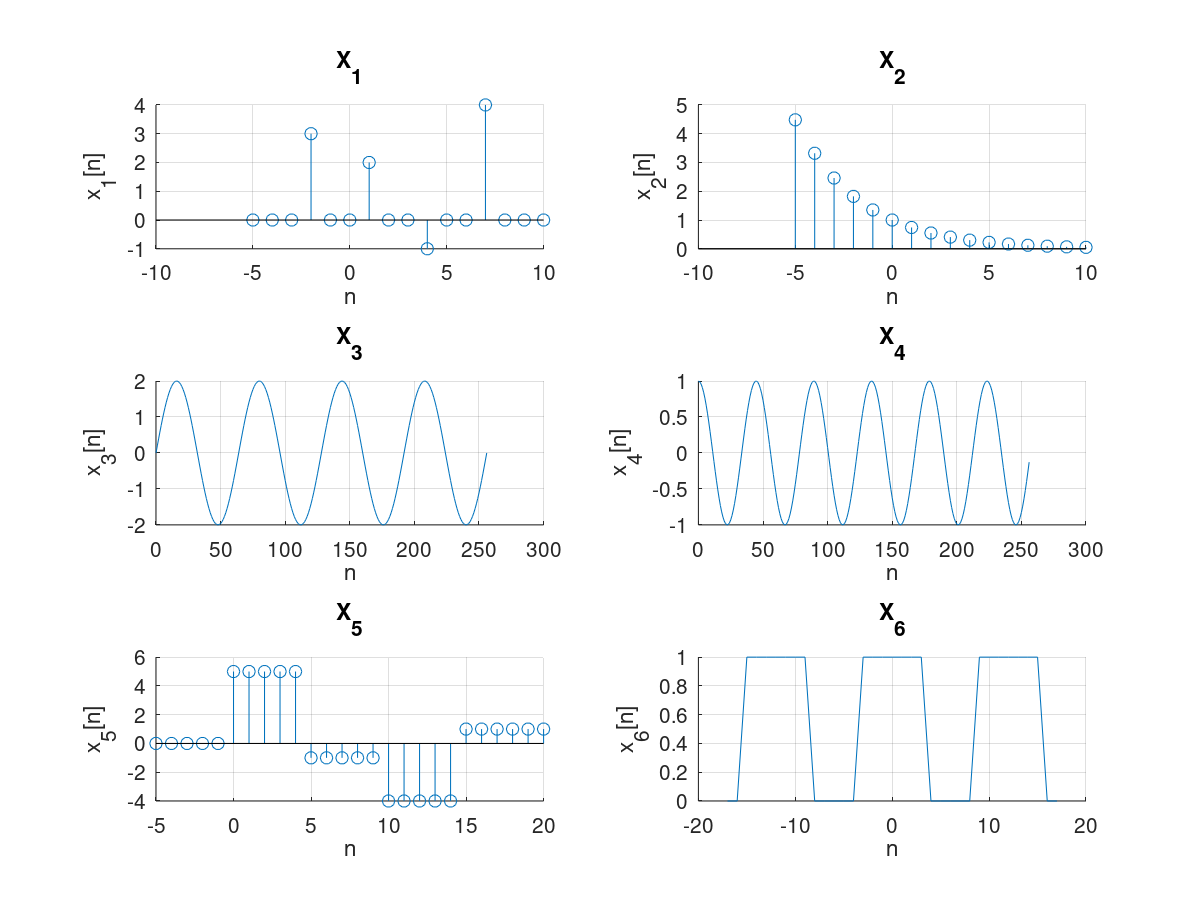
\includegraphics{x1_6.png}
    }
    \subsection*{b}
    \begin{itemize}
        \item $x_3 \rightarrow f_0 = \frac{\frac{2\pi}{64}}{1} \Rightarrow  \Omega_0 = \frac{2\pi}{64}$
        \item $x_4 \rightarrow f_0 = \frac{9}{64*2\pi} \Rightarrow \frac{9}{64}$
    \end{itemize}
    \subsection*{c}
    \begin{itemize}
        \item $x_3$ ist periodisch, die Periodendauer ist abzulesen bei x= 64.
        \item $x_4 \rightarrow n = \frac{2\pi k}{\frac{9}{64}}\Rightarrow \frac{2\pi * 64 k}{9}$ \\k müsste eine irrationale Zahl sein damit n ein Element aus den ganzen Zahlen ist. Zu diesem diskreten Punkt gibt es keine Periodendauer. 
    \end{itemize}
    \subsection*{d}
    \section*{3}
    Der Durchschnitt unserer Dreiecksfunktion ist $0$ was leicht anhand der Symmetrie bezüglich der x-Achse gesehen werden kann. Damit ist auch der DC-Anteil der Fourierreihe, $a_0$, $0$.
    Dies kann auch folgendermassen gezeigt werden :
    
    \begin{eqnarray*}
        a_{0} &=\frac{1}{T}\int_{0}^{T}f(t)dt 
    \end{eqnarray*}

Aufgrund der Symmetrie in der Funktion erkennen wir dass das Integral von $0$ nach $\frac{T_0}{2}$ gleich dem Integral von $\frac{T_0}{2}$ nach $T_0$ sein muss. Daher können wir sagen dass :
\begin{equation}
    a_0=\frac{2}{T_0}\int_{0}^{\frac{T_0}{2}}f(t)dt 
\end{equation}

Wir können uns nun auf einen Teil der zweiteiligen Funktion beschränken. Da die Funktion an der Strecke von $0$ nach $\frac{T}{2}$ die Form $A-\frac{4A}{T}$ hat gilt :
\begin{eqnarray*}
    a_0=&\frac{2}{T_0}\int_{0}^{\frac{T_0}{2}}A-\frac{4A}{T_0}tdt \\
    =&\frac{2}{T_0}(At-\frac{4A}{T_0}\frac{t^2}{2})\big |_0^{\frac{T_0}{2}}\\
    =&\frac{2}{T_0}(A\frac{T_0}{2}-\frac{2A\frac{T_0^2}{4}}{T_0}-A0-\frac{2A\frac{0}{4}}{T_0})\\
    =&\frac{2}{T_0}(A\frac{T_0}{2}-\frac{AT_0^2}{2T_0}-0-0)\\
    =&\frac{2}{T_0}(A\frac{T_0}{2}-A\frac{T_0}{2}-0) \\ =& \underline{0}
\end{eqnarray*}

\pagebreak

    Um $a_n$ zu finden können wir, wieder aufgrund der oben festgestellten Symmetrie, folgenden Term evaluieren :
    \begin{eqnarray*}
        a_n = & \frac{4}{T}\int_{0}^{\frac{T}{2}}f(t)\cos\omega ntdt\\
        =&\frac{4}{T}\int_{0}^{\frac{T}{2}}(A-\frac{4A}{T}t)\cos\omega ntdt \\
        =&\frac{A4}{T}\int_{0}^{\frac{T}{2}}(1-\frac{4}{T}t)\cos\omega ntdt \\
        =&\frac{A4}{T}(\int_{0}^{\frac{T}{2}}\cos\omega ntdt-\int_{0}^{\frac{T}{2}}\frac{4}{T}t\cos\omega ntdt)\\
        =&\frac{A4}{T}((\frac{1}{\omega n}\sin\omega nt)\big |_0^{T}-\int_{0}^{\frac{T}{2}}\frac{4}{T}t\cos\omega ntdt)\\
        =&\frac{A4}{T}((\frac{1}{\omega n}\sin\frac{2\pi}{T} n\frac{T}{2}-(\frac{1}{\omega nt}\sin\frac{2\pi}{T} n 0)-\int_{0}^{\frac{T}{2}}\frac{4}{T}t\cos\omega ntdt)\\
        =&\frac{A4}{T}((\frac{1}{\omega n}\sin \pi n- 0 -\int_{0}^{\frac{T}{2}}\frac{4}{T}t\cos\omega ntdt)
    \end{eqnarray*}
    Ganzzahlige Vielfache von pi ergeben immer einen Sinus von 0.
    \begin{eqnarray*}
        a_n = & \frac{A4}{T}(0 - 0 -\int_{0}^{\frac{T}{2}}\frac{4}{T}t\cos\omega ntdt)\\
         = & \frac{A4}{T}\int_{0}^{\frac{T}{2}}\frac{-4}{T}t\cos\omega ntdt\\
         = & \frac{-16A}{T^2}\int_{0}^{\frac{T}{2}}t\cos\omega ntdt\\
         = & \frac{-16A}{T^2}((t \frac{1}{\omega n}\sin \omega n t)\big |_0^\frac{T}{2}-\int_0^{\frac{T}{2}}\frac{1}{\omega n}\sin \omega ntdt)\\
         = & \frac{-16A}{T^2}(( \frac{\frac{T}{2}}{\omega n}\sin \frac{2\pi}{T} n \frac{T}{2} - \frac{1}{\omega n}\sin 0) -\int_0^{\frac{T}{2}}\frac{1}{\omega n}\sin \omega ntdt)\\
         = & \frac{-16A}{T^2}(( \frac{\frac{T}{2}}{\omega n}\sin \pi n -  0) -\int_0^{\frac{T}{2}}\frac{1}{\omega n}\sin \omega ntdt)\\
         = & \frac{-16A}{T^2}( 0 -\int_0^{\frac{T}{2}}\frac{1}{\omega n}\sin \omega ntdt)\\
         = & \frac{16A}{T^2}(\frac{-1}{\omega^2 n^2}\cos\omega n t )\big |_0^{\frac{T}{2}}\\
         = & \frac{16A}{T^2}\frac{1}{\omega^2 n^2}(-\cos\omega n t )\big |_0^{\frac{T}{2}}\\
         = & \frac{4A}{\pi^2 n^2}(-\cos\frac{2\pi}{T}n\frac{T}{2}+\cos 0)\\
         = & \frac{4A}{\pi^2 n^2}(-\cos\pi n + 1)
    \end{eqnarray*}

    Bei ungeraden Werten von n evaluiert dieser Term zu $\frac{8A}{\pi^2 n^2}$ bei geraden zu $0$ da der Cosinus bei ungeraden Vielfachen von $\pi -1$ annimmt und bei geraden 1. 


    Der Faktor $b_n$ ist bei geraden periodischen Funktionen, d.h. periodischen Funktionen die symmetrisch zur y-Achse sind, immer 0.
    
    Eingesetzt in die Fourierreihe erhalten wir nun.

    \begin{eqnarray*}
        x(t) = &  \sum_{n=1}^\infty \frac{8A}{\pi^2 (2n-1)^2}\cos(2\pi (2n-1) f_0 t)
        =& \frac{8A}{\pi^2}\sum_{n=1}^\infty\frac{\cos(2\pi (2n-1) f_0 t)}{(2n-1)^2}
    \end{eqnarray*}

    $n$ schreitet voran als $2n-1$ da wir nur an ungeraden Werten interessiert sind.

    \end{document}